\documentclass{article}
\usepackage[utf8]{inputenc}

\usepackage{amsmath}
\usepackage{hyperref}

\title{ECE220 Final Review - Cramming Carnival}
\author{Author: Members of HKN}
\date{Fall 2024}

\newcommand{\dd}[1]{\mathrm{d}#1}

\usepackage[makeroom]{cancel}
\usepackage[letterpaper, portrait, margin=1in]{geometry}
\usepackage{graphicx}
\usepackage{float}
\usepackage{enumitem}
\usepackage{graphicx}
\usepackage{multicol}
\usepackage{xcolor}
\usepackage{listings}

\definecolor{mGreen}{rgb}{0,0.6,0}
\definecolor{mGray}{rgb}{0.5,0.5,0.5}
\definecolor{mPurple}{rgb}{0.58,0,0.82}
\definecolor{backgroundColour}{rgb}{1,1,1}
\newcommand{\wideunderscore}{\underline{\hphantom{n}}}

\lstdefinestyle{CStyle}{
    backgroundcolor=\color{backgroundColour},   
    commentstyle=\color{mGreen},
    keywordstyle=\color{magenta},
    numberstyle=\tiny\color{mGray},
    stringstyle=\color{mPurple},
    basicstyle=\footnotesize,
    breakatwhitespace=false,         
    breaklines=true,                 
    captionpos=b,                    
    keepspaces=true,                 
    numbers=left,                    
    numbersep=5pt,                  
    showspaces=false,                
    showstringspaces=false,
    showtabs=false,                  
    tabsize=2,
    language=C,
    escapechar=\@
}

\pagenumbering{arabic}

\begin{document}

\maketitle

\section{
Logical Little Computer 3 Language Lessons}
\begin{enumerate}[label=(\alph*), itemsep = 120pt]
    \item \textbf{I/O}: What is the difference between Polling I/O versus Interrupt I/O?
    

    \item \textbf{Stack}: When using a stack, when you pop an item off the stack, is it removed from memory?

    
    \item \textbf{Stack Pt. 2}: If the input stream to a Stack is 123456789, design a set of pushes and Pops such that it is outputted 235641897?
    
    \item \textbf{Subroutines}: What is the purpose of using subroutines in LC3?
    
    \item \textbf{Multiplication}: Write a Multiplication Subroutine in LC3 assembly language.
    \newline
    ;input R3, R4 \newline
    ;out R0 \newline
    MULTIPLY \newline
    ;your code goes here: \newline
    \newpage

    
     \item 
    \textbf{More subroutines}: What extra step do you need to take when executing a subroutine inside a subroutine? (Hint: What gets overwritten when JSR is called?)
    
    \end{enumerate}

   

\newpage
\section{Captivating C Coding}
\begin{enumerate}[label=(\alph*), itemsep = 120pt]
    \item \textbf{Variable lifespan}: Explain the “lifespan” of a local variable during a C function call.
    
    
    \item \textbf{Poopy Pointers}: Explain the importance of having the parameters of this function being pointers.
    
    \begin{lstlisting}[style=CStyle]
void swap(int* a, int* b)
{
    int temp;
    temp = *a;
    *a = *b;
    *b = temp;
} \end{lstlisting}

    
 
    \item \textbf{Lovely Linked Lists}: What is the benefit of using a linked list over an array to represent a large, ever-changing list?
    
    \item \textbf{Rambunctious Recursion}: When writing a recursive algorithm, what is the goal of each recursive step? (Hint: The base case represents the simplest form of the problem)
    
    \item \textbf{Arrays}: How are arrays passed into functions in C?
    
    \item \textbf{Static Silliness}:  What is printed by the following program?
    \begin{lstlisting}[style=CStyle] 
static char letters[6] = {'A', 'E', 'F', 'D', 'B', 'C'};

void mystery () {
    static int X = 5;
    int Y = 2;
    printf ("%c%c", letters[--Y], letters[X--]);
}
int main() {
    mystery();
    mystery();
    return 0;
}
 \end{lstlisting}
    
    \item \textbf{Midpoint}: What is wrong with this recursive midpoint function?
\begin{lstlisting}[style=CStyle] 
find@\wideunderscore@midpoint(int a, int b) {
    if (a == b) { return a; }
    else if (a < b){
       return find_midpoint (a+1, b-1);
    } 
    else if (a > b){
       return find_midpoint( a-1, b+1); 
    } 
}\end{lstlisting}  
    \newpage
    \item \textbf{Function Foo}: What is this function accomplishing? Assume it is called with a valid head to a singly linked list.
\begin{lstlisting}[style=CStyle] 
struct node{
    int num;
    struct node* next;
}
int foo(struct node* head, int bar) {
    if (head->num >= bar) {
        bar = head->num;
    }
    if (head->next == null) {
        return bar;
    }
    else {
        return foo(head->next, bar);
    }
}\end{lstlisting}  
    \item Which sorting algorithm is this?
\begin{lstlisting}[style=CStyle]
void sort(int arr[], int n) {
    int i, j;
    for (i = 0; i < n - 1; i++)
        for (j = 0; j < n - i - 1; j++)
            if (arr[j] > arr[j+1])
                swap(&arr[j], &arr[j + 1]);
}\end{lstlisting}

    \newpage
    \item \textbf{Binary Search Trees}: Are these binary search trees?
    
    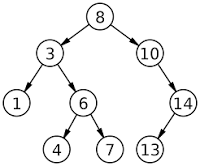
\includegraphics[width=7cm,height=6cm]{figures/bst.png}
    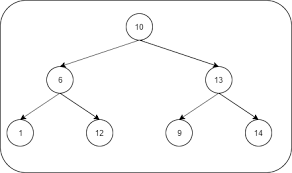
\includegraphics[width=7cm,height=6cm]{figures/notbst.png}
    
    \item \textbf{C to LC3}: Convert the following C function into LC3 using Callee Setup and Teardown.
    \begin{lstlisting}[style=CStyle] 
int foo(int a, int b) {
    int x;
    x = a + b;
    return x;
}\end{lstlisting}
    \newpage
    \item \textbf{Recursive Reversal}: What is the output of this program? If there is an error in ReverseArray, identify the line and fix it? (Hint: it might be nice and helpful to print every step of Reverse Array)
    
\begin{lstlisting}[style=CStyle] 
void ReverseArray(int array[], int size) {
    int start = 0;
    int end = size - 1;
    int temp;
    
    if (start < end) {
        // Swap First and Last
        temp = array[start];
        array[start] = array[end];
        array[end] = temp;
        
        ReverseArray(array, size-1);
    }
}
int main(){
    int array[5], i;
    for (i = 0; i<5; i++){
        array[i] = i;
    }
    ReverseArray(array, 5);
    printf("Reversed Array: ");

    for (i = 0; i<5; i++){
        printf("%d ", array[i]);
    }
    printf("\n");
    return 0;
}\end{lstlisting}

\item \textbf{}What is wrong with the following code? 
\begin{lstlisting}[style=CStyle] 
double * firstlast(const double values[], int size)
{
    double result[2];
    result[0] = value[0];
    result[1] = value[size-1];
    return result;
}
\end{lstlisting}

\item \textbf{Alternative Indexing}: Fill in the blanks to make the two arrays the same. Assume row-major order for array2.
\begin{lstlisting}[style=CStyle] 
int array1[4][2];
int array2[8];
int i, j;
for (i = 0; i < 2; i++) {
    for(j = 0; j < 4; j++) {
    array1[  ][  ] = i + j;
    array2[     ] = i + j;
    }
}
\end{lstlisting}

\item Fill In the blanks to find the student with the highest GPA and store a pointer to them in best\_student
\begin{lstlisting}[style=CStyle] 
typedef struct StudentStruct {
    int UIN;
    float GPA;
} Student;

int main () {
    Student all_students[5];
    // Load data into all students:
    load_students(all@\wideunderscore@students, 5);
    // Find the student with the highest GPA:
    Student* best@\wideunderscore@student = 
    find@\wideunderscore@best(all@\wideunderscore@students, 5,         );
    printf("Best GPA:%f\n",         );
}

void find@\wideunderscore@best(Student* all, int num@\wideunderscore@students, Student** best) {
    for (int i = 0; i < num@\wideunderscore@students; i++) {
        if (all[i].GPA >        ) {
            // Fill:
        }
    }
}

\end{lstlisting}

\item In MP10, we tasked you with inserting a node into a sorted singly-linked list. To help you get accustomed to poopy pointer arithmetic, we will now attempt to do the same, but with a doubly-linked list. You are given the following struct doubly\_node and the function insert\_doubly\_node(), which takes in the head of a doubly linked list (but you will not have a tail) and a value to insert. Complete the function skeleton below. Assume that the double-pointer head is never NULL, but that the single pointer *head (the result of dereferencing head once) is not necessarily never NULL.

\begin{lstlisting}[style = CStyle]
    typedef struct doubly@\wideunderscore@node {
        int value
        doubly@\wideunderscore@node * next;
        doubly@\wideunderscore@node * prev;
    } doubly@\wideunderscore@node;


    void print@\wideunderscore@list@\wideunderscore@d(doubly@\wideunderscore@node * head)
    {
        doubly@\wideunderscore@node * cur = head;
        while (cur != NULL)
        {
            printf("%d -> ", cur->value);
            cur = cur->next;
        }
    }

    void insert@\wideunderscore@doubly@\wideunderscore@node(doubly@\wideunderscore@node ** head, int value) 
    {
        /* edge case 0: linked list is completely empty */
        if(*head ==         ) 
        {
            *head = (             ) malloc(sizeof(          ));
            (*head)->next =         ;
            (*head)->prev =         ;
            (*head)->value =         ;
            return;
        }

        /* edge case 1: insert AT the head*/
        if (value < (*head)->      )
        {
            doubly@\wideunderscore@node * new@\wideunderscore@node = (          ) malloc(          );
            new@\wideunderscore@node->        = value;
            new@\wideunderscore@node->next =            ; //new node should be inserted before head
            new@\wideunderscore@node->          = NULL; //new node previous does not point to anything
            (*head)->        =  new@\wideunderscore@node; //head's previous points to new@\wideunderscore@node
            *head =          ; //update the new head of the linked list
            return;
        }

        doubly@\wideunderscore@node * cur = *head;
        while (cur !=      )
        {
            if (cur->value < value)
            {
                /* last edge case: insert AFTER the tail of the linked list */
                if (cur->next == NULL)
                {
                    doubly@\wideunderscore@node * new@\wideunderscore@node =                                   ; 
                    //allocated new@\wideunderscore@node on the heap

                    new@\wideunderscore@node->value = value;
                    new@\wideunderscore@node->next =            ; //new@\wideunderscore@node is the tail of the list
                    new@\wideunderscore@node->      = cur; //new@\wideunderscore@node's previous points to the current
                    cur->next =      ; //cur's next is the new node
                    return;
                }
            cur =            // advance to the next node
            }
        
        

            else 
            {
                doubly@\wideunderscore@node * new@\wideunderscore@node = (       ) malloc(sizeof(       ));
                new@\wideunderscore@node->value =            ;
                new@\wideunderscore@node->next =             ;
                new@\wideunderscore@node->         = cur->prev;
                cur->prev->next =        ;
                cur->prev = new_node;
                return;
            }
        }
    }
\end{lstlisting}

Assuming that insert\_doubly\_node() and print\_list\_d() are implemented correctly, what will the output of this code snippet be? 

\begin{lstlisting}[style = CStyle]
    int main()
    {
        doubly@\wideunderscore@node * head = NULL;
        insert@\wideunderscore@doubly@\wideunderscore@node(&head, 5);
        insert@\wideunderscore@doubly@\wideunderscore@node(&head, 2);
        insert@\wideunderscore@doubly@\wideunderscore@node(&head, 7)
        insert@\wideunderscore@doubly@\wideunderscore@node(&head, 9);
        insert@\wideunderscore@doubly@\wideunderscore@node(&head, 1);
        insert@\wideunderscore@doubly@\wideunderscore@node(&head, 10);
        insert@\wideunderscore@doubly@\wideunderscore@node(&head, 5);
        print@\wideunderscore@list@\wideunderscore@d(head);

        return 0;
    }
\end{lstlisting}

\end{enumerate}
\newpage
\section{C++ Programming}

\begin{enumerate}[label=(\alph*), itemsep = 120pt]
    \item \textbf{Class}: What is the difference between structs in C and classes in C++?
    
    \item \textbf{Constructor}: What does a constructor do in a class? What does a destructor do in a class? What might happen if we do not have a correct destructor?
    
    \item \textbf{Access specifier}: What is the difference between public, private, and protected in a C++ class?
    
    \item \textbf{Operator overloading}: What does operator overloading do in a C++ class? Give four different examples of operators that can be overloaded.
    
    \item \textbf{Rectangle}: Write the constructors and area function for this rectangle class.
    \begin{lstlisting}[style=CStyle]
class Rectangle {
private:
    int width, height;
public:
    Rectangle();
    Rectangle(int w, int h);
    int const area();
}
\end{lstlisting}
    \item \textbf{Iterator}: What will be printed if we run the following C++ code? (assume we import all needed files)
    \begin{lstlisting}[style=CStyle]
    int main() 
{ 
    vector<int> ar = { 1, 2, 3, 4, 5 }; 
    vector<int>::iterator ptr = ar.begin(); 
    ptr++;
    cout << *ptr << endl; 
    ptr = ptr + 3;
    cout << *ptr << endl; 
    return 0; 
}
\end{lstlisting}
    \item \textbf{Template}: What will happen if we run the main function?
    \begin{lstlisting}[style=CStyle]
template <typename T>
T max(T x, T y)
{
    return (x > y)? x : y;
}
int main()
{
    cout << max(3, 7) << endl;
    cout << max(3.0, 7.0) << endl;
    cout << max(3, 7.0) << endl;
    return 0;
}
\end{lstlisting}
    \item \textbf{Copy}: What is the difference between shallow copy and deep copy?


    \item \textbf{} What type of traversal is this?
    \begin{lstlisting}[style=CStyle]
void traversal (node *root) {
    if ( root != NULL) {
       std::cout << root -> data << std::endl;
       traversal (root -> left);
       traversal (root -> right);
    }
 }
    \end{lstlisting}

\item \textbf{}
What is the pre-order, in-order, post-order and level order traversal for the following binary search tree?

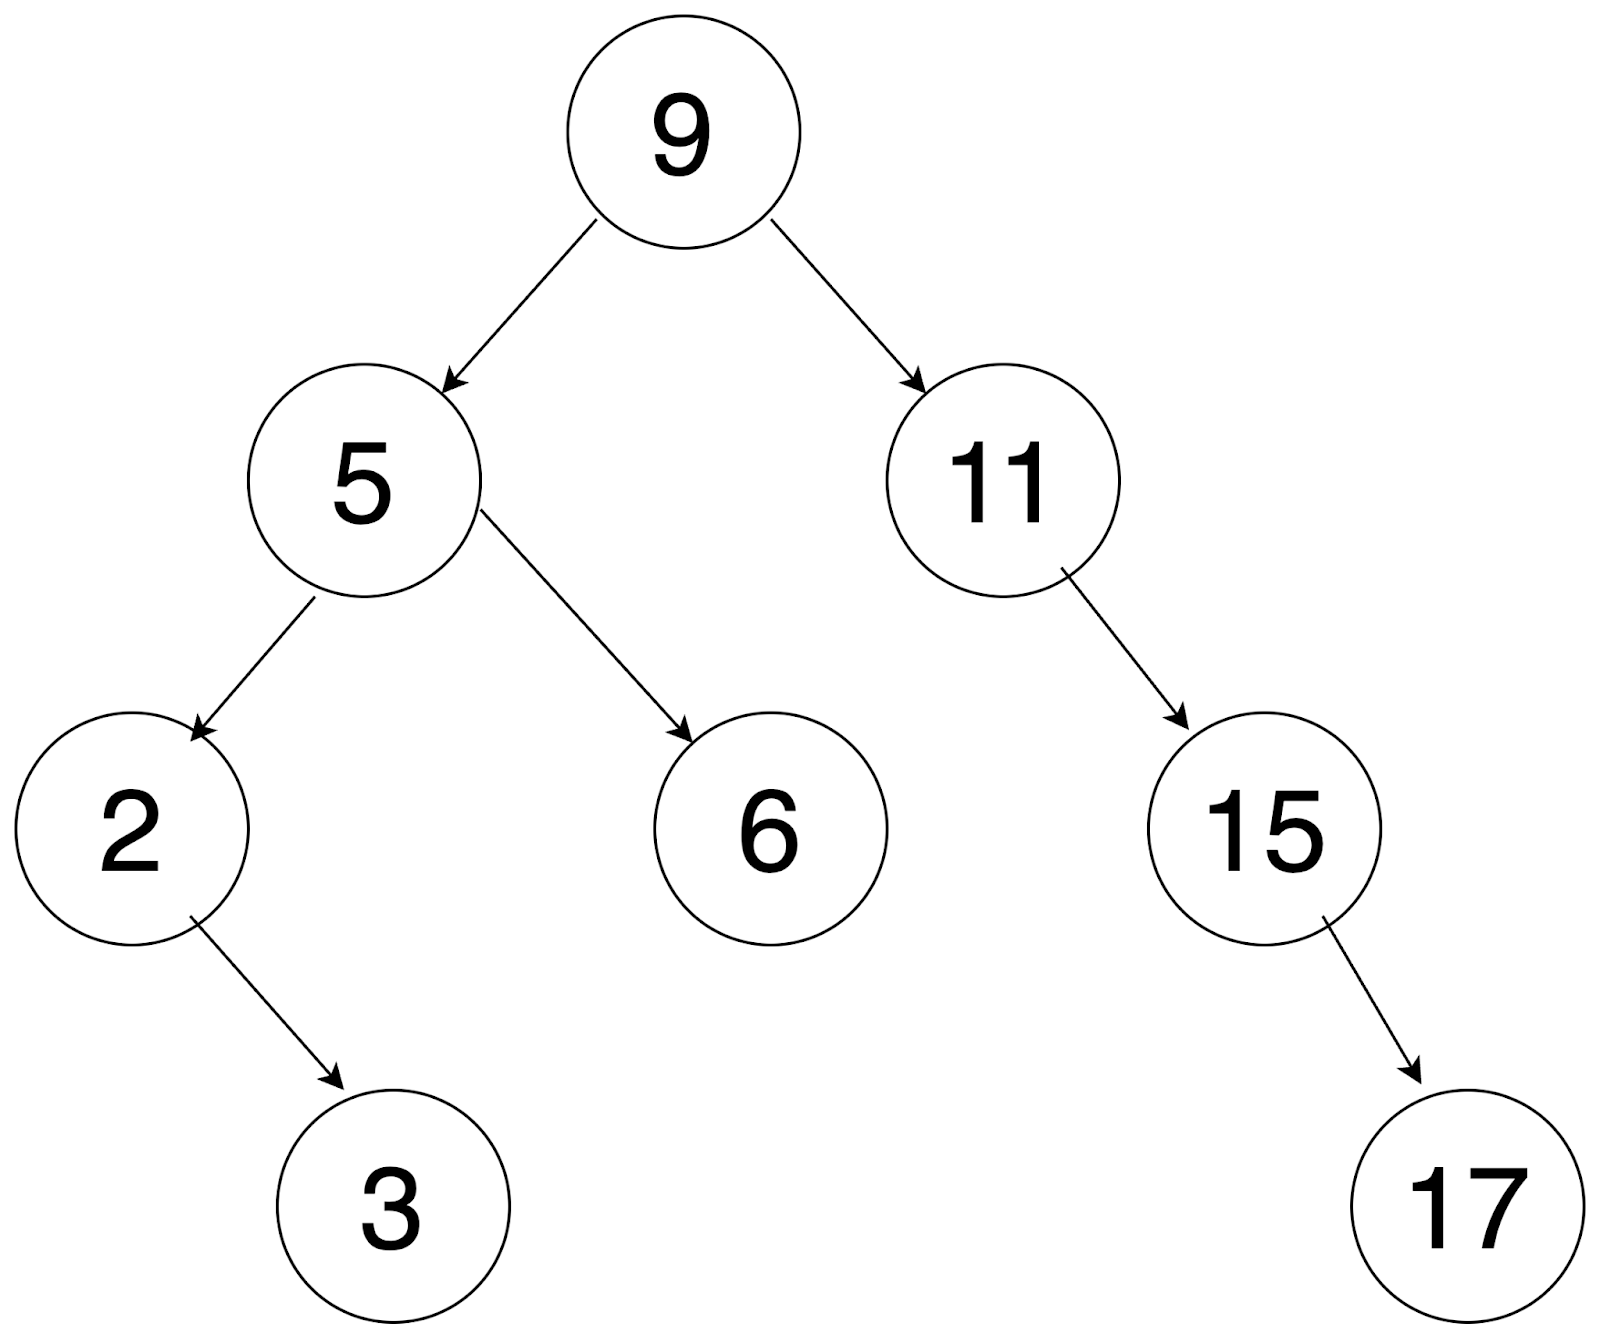
\includegraphics[scale = 0.125]{figures/bst2.png}


\item \textbf{}
How many bytes of memory have been allocated on the heap? Assume that we are in a 32-bit system (recall that an int is 4 bytes, a double is 8 bytes, an int * is 4 bytes, and a char is 1 byte)

    \begin{lstlisting}[style=CStyle]

    int main () {
        int a = 4;
        int d = 6;
        int c = 10; 
        int ** b = new int * [5];  
        b[0] = &a;
        b[1] = &c;   
        b[2] = &d;
        b[3] = new int[6];
        b[3][0] = 5;
        b[3][2] = 8;
        b[3][1] = 17;
        b[3][5] = 2;
        b[3][4] = 9;
        b[3][3] = 22; 
        b[4] = new int(13);
        char * character = new char (k);
 }


    \end{lstlisting}

    Write the contents of what each pointer points to (if it points to an array, write the contents of the array. If it points to a single int/char, write what the int/char is.) \newline \newline \newline \newline \newline 


Fill in the lines after line 10 needed to properly free the memory. Not all lines may be needed.

    \begin{lstlisting}[style=CStyle]
int main () {
    int a = 4;
    int d = 6;
    int c = 10;
    int ** b = new int * [5];  
    b[0] = &a;
    b[1] = &c;   
    b[2] = &d;
    b[3] = new int[6];
    b[3][0] = 5;
    b[3][2] = 8;
    b[3][1] = 17;
    b[3][5] = 2;
    b[3][4] = 9;
    b[3][3] = 22; 
    b[4] = new int(13);
    char * character = new char('k');
    ________
    ________
    ________
    ________
    ________
    ________
 }

    \end{lstlisting}

    Let’s say we have a void pointer p. What is the difference between delete [] p and delete p?



    \item Linked List Problem:
    Your best friend Gabriel has a C program that stores the name of his favorite Fortune 500 company. He is storing the company name in a linked list format. The structure of the linked list and the nodes are located below. The end of the list will have the company \wideunderscore node * next point to NULL;

    \begin{lstlisting}[style = CStyle]
        typedef struct company@\wideunderscore@node
        {
            int index;
            char letter;
            struct company@\wideunderscore@node * next;
            
        } company@\wideunderscore@node;

        typedef struct company
        {
            int n; //number of entries in list
            company@\wideunderscore@node * company_head;
            
        } company;
    \end{lstlisting}

    Given the above structure, and the fact that the company\wideunderscore node * pointer is 8 bytes (64-bit system),
    \textbf{what is the size in bytes of both struct company and struct company\wideunderscore node?}


    \vspace{2.5cm} %adding space for student answer
    
    Gabriel wants to tell you what his favorite Fortune 500 company is but is unable to speak because he just got his wisdom teeth removed. \textbf{Fill in the below program to print the name of the company.} This program takes place in main and has already imported the relevant libraries. 

    Assume everything has been initialized/malloc'd correctly and the name of the struct was declared with the following line. 

    Part 1: Printing

    \begin{lstlisting}[style = CStyle]
        company * gabriel@\wideunderscore@company;

        printf("The Name of Gabriel's Favorite Fortune 500 Company: ");

        company@\wideunderscore@ * current = gabriel@\wideunderscore@company->company@\wideunderscore@head;
        for (int i = 0; i < @\rule{1in}{0.5pt}@; i++) //iteraite through the list
        { 
            printf("%c", @\rule{1in}{0.5pt}@); //print the current character
            @\rule{1in}{0.5pt}@ //move the current node
        }
    \end{lstlisting}
    
    Gabriel is quite shy and doesn't want anyone to know what his favorite Fortune 500 company is (except for you, his best friend). \textbf{Help him finish the below code to remove the company name from the heap.}

    Part 2: Freeing
    \begin{lstlisting}[style = CStyle]
        company@\wideunderscore@node * the@\wideunderscore@current = gabriel@\wideunderscore@company->company@\wideunderscore@head;
        company@\wideunderscore@node the@\wideunderscore@previous = gabriel@\wideunderscore@company->company@\wideunderscore@head;
        while(the@\wideunderscore@current->next != @\rule{2in}{0.5pt}@){
            the@\wideunderscore@current = the@\wideunderscore@current->next;
            free(@\rule{2in}{0.5pt}@);
            @\rule{2in}{0.5pt}@; //move previous further
        }

        free(gabriel@\wideunderscore@company);
    \end{lstlisting}

    Whenever the above code is executed, a memory leak occurs. /textbf{Explain what a memory leak is and come up with one line of code that can be added above to fix the memory leak.}

    \item Virtual Keywords:
    \begin{lstlisting}[style = CStyle]
        #include <iostream>
        class Base
        {
            public: 
                virtual void f()
                {
                    std::cout << "base\n";
                }
        };

        class Derived@\wideunderscore@One : public Base
        {
            public:
                void f() override
                {
                    std::cout << "derived_1\n";
                }
        };

        class Derived@\wideunderscore@Two : public Base 
        {
            public: 
                void f()
                {
                    std::cout << "derived_2\n";
                }
        };

    
        int main()
        {
            //Define the objects
            Base b;
            Derived@\wideunderscore@One d@\wideunderscore@1;
            Derived@\wideunderscore@Two d@\wideunderscore@2;

            //assign the objects by reference
            Base& br = b;
            Base& dr@\wideunderscore@1 = d@\wideunderscore@1;
            Base& dr@\wideunderscore@2 = d@\wideunderscore@2;

            /* PART 1 */
            br.f();
            dr@\wideunderscore@1.f();
            dr@\wideunderscore@2.f();

            //Assign the objects by pointer
            Base * bp = &b;
            Base * dp_1 = &d@\wideunderscore@1;
            Base * dp_2 = &d@\wideunderscore@2;

            /* Part 2 */
            bp->f();
            dp@\wideunderscore@1->f();
            dp@\wideunderscore@2->f();

            /* Part 3 */
            br.Base::f();
            dr@\wideunderscore@1.Base::f();
            dr@\wideunderscore@2.Base::f();

            return 0
        }
    \end{lstlisting}
    Part 1:
    What is printed by br, dr\_1, and dr\_2?

    \vspace{2cm}
    Part 2:
    What is printed by br, dr\_1, and dr\_2? What is the difference between Part 1 and Part 2?

    \vspace{2cm}
    Part 3:
    What is printed br, dr\_1, and dr\_2? What is the difference between the other two parts?
    \vspace{2cm}
    
    \end{enumerate}


    
\end{document}